\section{Evaluation}
\label{sec:eval}
\subsection{Simulation setup}
The read is evaluated on an 8$\times$8 slice of the layout netlist of the macro, with its drivers, word-line flip-flops and level shifters, drain switches, delay line, and TDC flip-flops, simulated with the foundry PSP models at the typical corner; process corners and temperature follow in Section~\ref{sec:rows}.
The cells are linear resistors, 9\,k$\Omega$ for the LRS and 200\,k$\Omega$ for the HRS, the top of the range IHP has characterized (1\,\si{\micro\ampere} at 0.2\,V), with 1\,M$\Omega$ added as an ideal case that a deeper reset would approach.
At the 0.06 to 0.12\,V the read places across a cell, the HRS non-linearity of these devices raises $R$ by about 10\,\% over its 0.2\,V value and the LRS is ohmic~\cite{zanotti2026model}, and at the two states the IHP compact model can produce (1.4 and 12\,k$\Omega$) it reproduces the crossing times of the resistor runs within 0.06\,ns.
The supplies are confined to $\Vd,\Vg,\Vdel\in\{0.8,0.9,1.0\}$\,V so that a read never approaches a write condition.

A resistor cell omits two capacitances that set the discharge, and both are added explicitly.
The first is the line loading, for which an RC extraction of the full macro (21\,930 transistors and 4096 MEMRES devices) gives 47 to 62\,fF of interconnect on each bit line and 21 to 36\,fF on each source line, so the slice adds 70\,fF to BL and 30\,fF to SL for the wire and the source junctions of the 56 rows it does not instantiate.
The second is the MEMRES stack itself, a metal-insulator-metal capacitor that neither the compact model nor the extraction contains.
For its design-rule area of 0.36\,\si{\micro\meter\squared}, 6\,nm of HfAlO, and $\varepsilon_\mathrm{r}=12$ to 20, a Sentaurus solution of the drawn stack gives $C_\mathrm{MIM}=6.8$ to 11.0\,fF per cell, and all results use 10\,fF.
This capacitance bypasses a selected cell with a time constant of 2\,ns at 200\,k$\Omega$ and 10\,ns at 1\,M$\Omega$, which is the scale of the differences the read resolves, and the line loading doubles every crossing time, so that all runs precharge for 40 cycles (400\,ns).

An access takes the precharge, the settle, the offset, and the READ pulse, about 0.45\,\si{\micro\second} for 512 result bits at 100\,MHz, and costs 8 to 13\,pJ per slice from the supply currents, or 65 to 105\,pJ per access scaled to the macro with the controller excluded (0.13 to 0.2\,pJ per bit).
Of this, 90\,\% is the clock energy of the word-line flip-flops, which toggle every cycle during the long precharge, so a clock gate during precharge would remove most of it, while the read path itself takes below 0.3\,pJ.

\subsection{Single-row read}
\begin{table}[!t]
\centering
\caption{Best operating point per operation (slice, LRS 9\,k$\Omega$)}
\label{tab:pim}
\scriptsize
\setlength{\tabcolsep}{1.6pt}
\begin{tabular}{@{}lccclcc@{}}
\toprule
op. & HRS & $\Vd/\Vg/\Vdel$ & off. & codes $c(k)$ & margin & $V_\mathrm{RRAM}$/$I_\mathrm{cell}$\\
 & ($\Omega$) & (V) & (ns) & $k=0\ldots8$ & (taps) & (V/\si{\micro\ampere})\\
\midrule
read, 1 row & 200\,k & 0.8/0.8/0.8 & 20 & 8, 0 (HRS, LRS) & 8 & 0.09/1.3\\
NOR, 8 rows & 200\,k & 0.9/0.8/1.0 & 10 & 7 1 0 0 0 0 0 0 0 & 6 & 0.06/0.8\\
majority, 8 rows & 200\,k & 1.0/0.8/1.0 & 10 & 8 8 8 6 3 1 0 0 0 & 2 & 0.06/0.8\\
NOR, 8 rows & 1\,M$^\dagger$ & 0.8/0.8/0.9 & 10 & 8 0 0 0 0 0 0 0 0 & 8 & 0.12/1.0\\
majority, 8 rows & 1\,M$^\dagger$ & 1.0/0.8/1.0 & 10 & 8 8 8 8 7 3 0 0 0 & 4 & 0.12/1.0\\
\midrule
\multicolumn{7}{@{}l}{direct transients, $C_\mathrm{MIM}=10$\,fF, extracted line capacitance; $^\dagger$ideal HRS}\\
\bottomrule
\end{tabular}

\end{table}
At $\Vg=0.8$\,V the access transistor is in weak inversion and limits the cell current to 0.5 to 1.7\,\si{\micro\ampere} (for 200 to 9\,k$\Omega$ with 0.9\,V on BL), so the 22:1 resistance ratio of the cells reaches the bit line as a current contrast of only 3 to 3.6:1.
Even so, a single row separates HRS from LRS by the full eight taps (Table~\ref{tab:pim}).
With all supplies at 0.8\,V the 200\,k$\Omega$ cell crosses the buffer threshold 50.7\,ns after the source line is grounded and the LRS cell after 28.2\,ns, a window at a +20\,ns offset lies between them, and the cell sees 0.09\,V and 1.3\,\si{\micro\ampere} during the read.

\subsection{Multi-row NOR and majority}
\label{sec:pim}
\begin{figure}[!t]
\centering
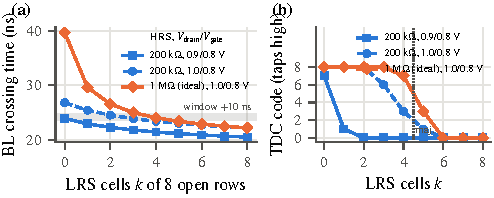
\includegraphics[width=\columnwidth]{grid}
\caption{8-row read with $k$ cells in the LRS, at 200\,k$\Omega$ and 1\,M$\Omega$ HRS: (a) bit-line crossing time, with the +10\,ns window shaded; (b) simulated TDC code.}
\label{fig:pim}
\end{figure}
Because $\Vd$ stays at or below 1\,V, the settle cycle must ground SL (the settle-drain bit of the controller), since with SL floating, charge sharing takes BL below the buffer threshold before READ.
The full supply grid was simulated for both HRS values, the codes at every window position were computed from the simulated crossing times and tap tables, and the best point of each operation was then simulated directly.
Table~\ref{tab:pim} lists these points and Fig.~\ref{fig:pim} shows the crossing times and codes behind them.

At 200\,k$\Omega$ every multi-row operation is resolved at $\Vg=0.8$\,V and at no higher word-line voltage, because the current-limited cells stretch the 8-row discharge band to 20 to 27\,ns (Fig.~\ref{fig:pim}(a)), wide enough for $\Vd$ to place it against the window grid, whereas at $\Vg\ge0.9$\,V the band is shorter than the 10\,ns offset step and falls between window positions.
At $\Vd=0.9$\,V the all-HRS crossing (23.9\,ns) lies inside the window and the $k=1$ crossing (22.9\,ns) before it, which gives the codes 7, 1, 0, \ldots\ of Fig.~\ref{fig:pim}(b) and a NOR margin of six taps, and the ideal 1\,M$\Omega$ reaches the full scale.
The majority is harder, because the step from $k$ to $k+1$ shrinks as $1/k^2$, so $c(4)-c(5)$ needs the window on the compressed part of the band; $\Vd=1.0$\,V moves it there and gives a majority by two taps, or four at 1\,M$\Omega$.
The 10\,ns step, one clock period, is thus the main limitation of the design, since it caps both the row count and the hot-corner margins that follow.

\subsection{Rows per access, corners, and temperature}
\label{sec:rows}
\begin{table}[!t]
\centering
\caption{Margin in taps vs.\ temperature at 200\,k$\Omega$, fixed / re-tuned setting}
\label{tab:retune}
\scriptsize
\setlength{\tabcolsep}{4pt}
\begin{tabular}{@{}lccc@{}}
\toprule
 & $-40$\,\si{\celsius} & 27\,\si{\celsius} & 125\,\si{\celsius}\\
\midrule
read, 1 row & 8 / 8 & 8 / 8 & 8 / 8\\
NOR, 8 rows & 0 / 5 & 5 / 5 & 0 / 1\\
majority, 8 rows & 0 / 2 & 2 / 2 & 0 / 0\\
\bottomrule
\end{tabular}
\end{table}
\begin{figure}[!t]
\centering
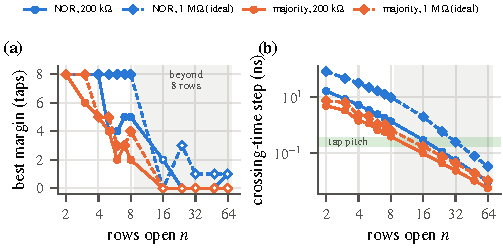
\includegraphics[width=\columnwidth]{rows}
\caption{Rows per access: (a) best NOR and majority margin; (b) crossing-time step behind each decision against the tap pitch (shaded). Hollow markers: at the best 8-row supplies.}
\label{fig:rows}
\end{figure}
Fig.~\ref{fig:rows} extends the same model from one to eight rows over the full supply grid, and to 16 to 64 rows at the best 8-row supplies.
At 200\,k$\Omega$ the NOR keeps all eight taps up to four rows and four to five taps up to eight, while the majority falls from eight taps at two rows to two or three at six to eight.
Every open row adds an HRS current against which one LRS cell must stand out, so the crossing-time step behind each decision falls roughly as $1/n^2$ (Fig.~\ref{fig:rows}(b)), from 17\,ns (NOR) and 5\,ns (majority) at two rows to 1.4 and 0.4\,ns at eight.
From 16 rows on, the step at 200\,k$\Omega$ is at or below a tap pitch, and the single-tap margins computed there are tap-edge artifacts.
One access therefore decides over at most eight rows at the characterized HRS, wider sums are split into eight-row groups that the host combines, and only two rows give a distinct code for every count.

Over the process corners and $-40$ to 125\,\si{\celsius} the 8-row band moves from 16 to 60\,ns against the 10\,ns window step, and this is where the tunability matters (Table~\ref{tab:retune}).
With the room-temperature setting held fixed, the 8-row operations are lost at both temperature extremes, whereas re-tuning $\Vd$, $\Vg$, $\Vdel$, and the offset per temperature keeps the single-row read at eight taps everywhere and recovers the 8-row NOR at $-40$\,\si{\celsius} with five taps, but not at 125\,\si{\celsius}, where the band is shorter than the step and one tap remains.

\subsection{Read disturb and the device budget}
A read biases the selected cells in the RESET polarity, with BL high and SL grounded, so repeated reads push the cells toward the HRS, and it is $\Vg$ rather than $\Vd$ that sets the stress.
At the best points a cell sees at most 0.06 to 0.12\,V and 0.8 to 1.3\,\si{\micro\ampere}, below the 0.2\,V read condition of the device and a sixth of its 8\,\si{\micro\ampere} RESET target.
On these devices $10^5$ pulses of 10\,\si{\micro\second} at 0.1 to 0.2\,V leave every level unchanged and drift starts at 0.3\,V, while retention alone lowers the LRS by 15\,\% in 100\,h at room temperature~\cite{baroni2026drift}, so the refresh interval is set by retention and temperature rather than by the read count.

The margins above hold at the typical corner with fixed resistances, and the final question is how much spread they tolerate.
With a 3 to 3.6:1 current contrast, a Monte Carlo analysis on the simulated crossing times, checked against 160 SPICE runs with drawn cell resistances, limits the HRS spread for an $n$-row decision at a $10^{-3}$ error rate to $\sigma_{\ln R}\approx0.46/\sqrt{n}$ with an ideal threshold, which is 0.46 for a single row, 0.33 for two rows, and 0.16 for eight.
Measured arrays show 0.3 to 0.6 on the 250\,nm devices and 0.5 to 1 on the Al-doped 130\,nm devices, whose HRS at the same verify has a median of 90 to 220\,k$\Omega$ but a conductive edge pinned at 50\,k$\Omega$~\cite{perez2017hfalo,baroni2025aldoping}.
The single-row read therefore works at the characterized HRS, whereas the 8-row logic needs the deeper reset of the 1\,M$\Omega$ rows of Table~\ref{tab:pim}, which buys a full-scale 8-row NOR, a four-tap majority, and an eight-row spread limit of 0.5, inside the measured range.
A deeper reset, a tighter verify window, and fewer rows per access are the levers, and a higher word-line voltage adds only 30 to 45\,\% of contrast.
The first two are programming-time costs, since a deeper reset takes more incremental-step-pulse-with-verify (ISPVA) pulses per write, about twelve of 12\,\si{\micro\second} at the 5\,\si{\micro\ampere} target~\cite{perez2017hfalo}, and with Al doping leaves a quarter of the cells at the read floor~\cite{baroni2025aldoping}, while a tighter window costs further verify iterations.

\subsection{Comparison and limitations}
\begin{table}[!t]
\centering
\caption{Comparison with RRAM and time-domain macros}
\label{tab:prior}
\scriptsize
\setlength{\tabcolsep}{1.7pt}
\begin{tabular}{@{}llllll@{}}
\toprule
 & node & memory & readout & summed$^\mathrm{a}$ & reported metric\\
\midrule
\cite{chen2018rram65nm} & 65\,nm & 1\,Mb 1T1R & current SA, 3\,b & 9--25 & 14.8\,ns/cycle\\
\cite{wan2022neurram} & 130\,nm & 3\,Mb 1T1R & ADC, calibrated & 256 & 43\,TOPS/W (1\,b)\\
\cite{sayal2020timedomain} & 40\,nm & none on chip & counter TDC & 25--150, serial & 12.1\,TOPS/W\\
\cite{xue2024tdcim} & 180\,nm & 8\,kb SRAM & counter TDC & 32 per chain & 0.3--0.8\,TOPS/W$^\mathrm{b}$\\
this work & 130\,nm & 4\,kb 1T1R & 8-tap TDC, tunable & $\le8$ & 0.13--0.2\,pJ/bit$^\mathrm{c}$\\
\bottomrule
\multicolumn{6}{@{}p{\columnwidth}@{}}{\scriptsize $^\mathrm{a}$cells sensed in one access; $^\mathrm{b}$8$\times$8\,b at 1.2\,V; $^\mathrm{c}$slice SPICE, 0.45\,\si{\micro\second} per access; SA: sense amplifier.}\\
\end{tabular}

\end{table}
Table~\ref{tab:prior} places the read next to the silicon RRAM and time-domain macros it draws on.
Those macros are MAC engines, so the table compares structure rather than figures of merit, and against their reference-tracked or calibrated readouts this work trades throughput for a bitwise read of up to eight rows whose every timing and drive level is a register or a pad.
The evaluation rests on an 8$\times$8 slice with resistor cells and a single value of $C_\mathrm{MIM}$, and its disturb bound rests on SET-polarity data, so the HRS spread and the RESET-polarity disturb are the first quantities to measure on silicon, while a fractional-cycle offset, which would lift the eight-row cap and the loss at 125\,\si{\celsius}, is the first change for a second version.
